\begin{document}
	\chapter{Dynamic Networks}

	
	\section{Complex Networks}
	
	Communication networks, transportation systems, social studies, biology and neuroscience all presents some characterization element that can be related to a social network. Social networks are structures were social actors interact with each other and through the \textit{social network analysis} it is possible to undergo deeply on the characterization of the network itself. While social network emerged as a prominent sociology topic in 1908 by Georg Simmel, it was later re-discovered by physicists and mathematically formalized in late 1950s. Through the years many researchers developed newer and more fine-grained models for these networks (Barabási–Albert\cite{Barabasi1999}, Erdős–Rényi\cite{Erdos1959}, Watts–Strogatz\cite{Watts1998}) producing a vast literature on the topic and several unique models that would capture essential properties of different scenarios.
	
	Social networks are usually complex networks, networks whose structure features non-trivial topology. Scale-free networks are of particular interest as they are random graphs (graphs whose degree distribution is regulated by a probability function) governed by a power-law probability function. The results is that in these particular networks some nodes exhibit a degree that can be order of magnitudes with respect to other nodes of the network. The terms scale-free was coined by Barabàsi and collaborators to indicate network whose probability distribution looks the same regardless the size of the network. The degree probability of a scale-free network is always defined as $$P(k) \sim k^{\gamma}$$ that is the probability for a node of a graph picked at random to have $k$ edges.
	
	The strict relationship between time and money in the Lightning Network puts it in an incredibly interesting spot regarding the dynamic properties of it: there must exist channels connecting pair of nodes along a payment path and every node involved in the payment path must be online in the moment a transaction is performed. A third constraint on a payment procedure is that every node involved in the payment process must have enough funds to transfer.
	
	The three constraints play a key role in the modeling of the network and put in evidence the dynamic feature of the network itself. Therefore the network is not a static entity but a dynamic one, and a lots of its feature will be shown have similarities with social networks. The dynamicity of a network has lately seen intensive research efforts and a vast literature is available, yet it often results to be very problem-specific and lacks of a universal formal description. An important contribution to this research area was the formalization of \textit{Time-Varying Graphs}\cite{Casteigts2012} that is a unified framework that address the main characteristics of a dynamic network, and whose goal is to put in evidence and formally define important concepts that were present in other research areas (delay-tolerant networks, opportunistic networks, real-world complex networks) but not related each other.
	
	
	\section{Time Varying Graph}

	A Time-Varying Graph (TVG) is described by a quintuple \(\text{TVG} = (V, E, T, \rho, \zeta) \):
	\begin{itemize}
		\item a set of nodes \(V\).
		
		\item a set of relations between nodes \(E\) (edges).	
		
		\item an alphabet \(L\) (optional).
		
		\item a relation \(E \subseteq V \times V \times L\) where \(L\) are domain-specific labels and can be used (or omitted) to enrich the description of the network.
		
		\item a time span *simbolo mancante* \( T \subseteq \mathbb{T}\) called \textit{lifespan} with \(\mathbb{T}\) representing the domain of time which usually coincides with the \(\mathbb{N}\) if the system is discrete, \(\mathbb{R}^+\) otherwise.
		
		\item a function \(\rho : E \times T \to \{0, 1\} \) called \textit{presence} to track the availability of an edge at a given time.
		
		\item a function \(\zeta : E \times T \to \mathbb{T}\) called latency function that indicates the time needed to cross an edge at a given date.
	\end{itemize}

	The model can also be enriched with two more functions that can capture the nodes dynamic behavior in a way similar to \(\rho\) and \(\zeta\).
	\begin{itemize}
		\item a function \(\psi : V \times T \to \{0, 1\}\) called \textit{node presence function}, expressing the availability of a node at a given time T.
		
		\item a function \(\phi : V \times T \to \mathbb{T}\) called 
	\end{itemize}
	
	Inside the definition of a time varying graph we have the notion of \textit{underlying graph}, that is the graph \(G = (V, E)\) which is the backbone of the dynamic network. One important thing to notice is that a connected component G doesn't imply the connectivity of the TVG, in fact the TVG could be disconnected for every time instant of its lifespan.
	
	\begin{figure}
		\begin{subfigure}{0.5\textwidth}
			\centering
			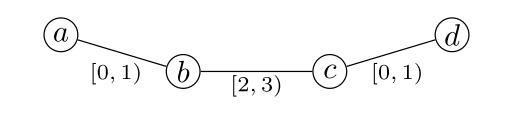
\includegraphics[scale=0.65]{example_tvg}
			\caption{The visual representation of a TVG.}
		\end{subfigure}
		\begin{subfigure}{0.5\textwidth}
			\centering
			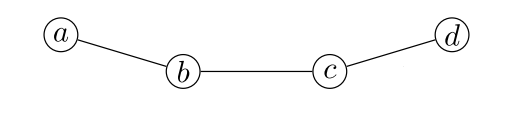
\includegraphics[scale=0.65]{example_underlying}
			\caption{The underlying graph.}
		\end{subfigure}
		\begin{subfigure}{0.5\textwidth}
			\centering
			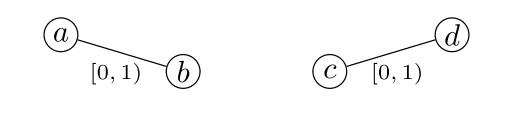
\includegraphics[scale=0.65]{example_tvg_0_1}
			\caption{Edges availability according to presence function at time interval [0, 1].}
		\end{subfigure}
		\begin{subfigure}{0.5\textwidth}
			\centering
			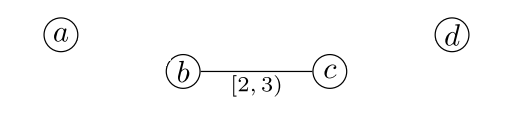
\includegraphics[scale=0.65]{example_tvg_2_3}
			\caption{Edges availability according to presence function at time interval [2, 3].}
		\end{subfigure}
		\caption{Layers of a Time Varying Graph. Image courtesy of \cite{Casteigts2012}.}
	\end{figure}
	
	\begin{itemize}
		\item \textit{Edge-centric evolution}: every edges has associated a set of the union of all the dates in which an edge \(e\) is available. Such set is denoted by \(I(e)\) and every element of \(I\) is such that \(I(e) = \{t \in T | \rho(e,t) = 1\}\), that is, the elements of the set are of the kind \(I(e) = \{t_1, t_2, t_3 ... \}\) and since they express time intervals it is possible to subdivide them in two sets \(App(e)\) and \(Dis(e)\), \textit{appearance and disappearance}, where \(App(e) = \{t_n | t_n \in I(e), n = 2N + 1\}\) and \(Dis(e) = \{t_n | t_n \in I(e), n = 2N\}\), i.e. every \(t\) in an even position is a date of appearance while \(t\) in odd position are dates of disappearance.
		
		\item \textit{Vertex-centric evolution}: nodes spawn and de-spawn causes changes in the configuration of the neighbor for some nodes, and it is expressed through \textit{sequences of neighborhoods} \(N_{t_1}(v), N_{t_2}(v), N_{t_3}(v) ...\). This kind of configuration is not very common in the literature.
		
		\item \textit{Graph-centric evolution}: it is the situation in which graphs are subject to events (edges appearance and disappearance) that make their topology change. Each of this events happens in a \textit{characteristic date}, and these dates are sorted in chronological such that \(S_{T}(\overline{G}) = sort(\cup\{S_t(e) : e \in E\})\) with \( \overline{G}\) being a TVG. From a global pont of view, it is possible to have a look at the evolution of the graph as a sequence of graph snapshot \(S_{\overline{G}} = G_1, G_2, G_3\) where \(G_i\) is a static snapshot of \(\overline{G}\) at time \(i\).
	\end{itemize}
	
	The time-varying graph framework also put emphasis on the different peculiarity of the different networks that can be modeled as a TVG by providing a classification method based on some particular properties. They are thirteen in total and are \textit{minimum reachability, all-nodes-reachability, connectivity over time, round connectivity, recurrent connectivity, recurrence of edges, time bounded recurrence of edges, periodicity of edges, constant connectivity, T-interval connectivity, eventual instant-connectivity, eventual instant-routability, complete graph of interaction}.
	Such a classification should help to categorize better a problem, and to help navigating the literature with well defined properties that have been investigated in other works.
\end{document}